\documentclass[a4paper,11pt,twoside]{scrartcl}
\usepackage[T1]{fontenc}
\usepackage{subcaption}
\usepackage[utf8]{inputenc}
\usepackage{ngerman, eucal, mathrsfs, amsfonts, bbm, amsmath, amssymb, stmaryrd,graphicx, array, geometry, color, wrapfig, float, hyperref, epstopdf,gensymb, subcaption, extarrows}
\usepackage[controls, step, poster=first]{animate}
\geometry{left=25mm, right=15mm, bottom=25mm}
\setlength{\parindent}{0em} 
\setlength{\headheight}{0em} 
\title{Graphenalgorithmen\\ Blatt 8}
\author{Markus Vieth\and Christian Stricker}
\date{\today}
\input{../head/lstlisting.tex}
\usepackage{float}
\usepackage[section]{placeins}
\usepackage{epstopdf}
\usepackage{wrapfig}
\usepackage{caption}
\usepackage{subcaption}
\usepackage{graphicx}
\usepackage{pgfplots}
\usepackage[usenames,dvipsnames,svgnames,table]{xcolor}
\usetikzlibrary{plotmarks}
\usetikzlibrary{patterns}
\usetikzlibrary{decorations.pathmorphing}
\usetikzlibrary{calc}
\usetikzlibrary{shapes}
\newcommand{\coloredcircled}[3][black]{{\large \Large\color{#2}\textcircled {{\small\color{#1}#3}}}}% Circlecolor, Textcolor, text
\newcommand{\ddvec}[2]{\begin{pmatrix}#1\\#2\end{pmatrix}}
\newcommand{\dddvec}[3]{\begin{pmatrix}#1\\#2\\#3\end{pmatrix}}
\newcommand{\longvec}[1]{\overset{\longrightarrow}{#1}}
\newcommand{\eunorm}[1]{\left\lVert#1\right\rVert_2}
\newcommand{\scalar}[2]{\left<#1,#2\right>}\newcommand{\cor}[1]{\textcolor{red}{\textit{#1}}}
\newcommand{\qed}{%
	\begin{flushright}
		q.e.d.
	\end{flushright}%
	}
\begin{document}
\maketitle
\cleardoublepage
\pagestyle{myheadings}
\markboth{Markus Vieth, Christian Stricker}{Markus Vieth, Christian Stricker}

\newpage
\section{Aufgabe 1: Separator im Graphen $G$ (10 Punkte)}
\section{Aufgabe 2: Cops and Robber (10 Punkte)}
\section{Aufgabe 3: Baumzerlegung berechnen (20 Punkte)}
\subsection{a}
\begin{figure}[H]
	\centering
	\begin{subfigure}{.33\textwidth}
		\centering
		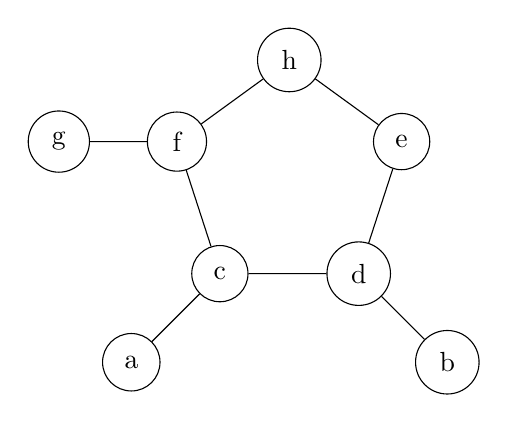
\begin{tikzpicture}[scale=1.5, every node/.style={draw,circle, align=center, inner sep = .5em}]
		\node at (90:1) (h) {h};
		\node at (90-72:1) (e) {e};
		\node at (90-72*2:1) (d) {d};
		\node at (90-72*3:1) (c) {c};
		\node at (90-72*4:1) (f) {f};
		\node at ($(f) + (-1,0)$) (g) {g};
		\node at ($ (c) - (.75,.75) $) (a) {a};
		\node at ($ (d) + (.75,-.75) $) (b) {b};
		\draw (g) -- (f) -- (h) -- (e) -- (d) -- (c) -- (f) (a) -- (c) (b) -- (d);
		\end{tikzpicture}
		\caption{Graph $G$}
	\end{subfigure}
	\begin{subfigure}{.66\textwidth}
		\centering
		\begin{tikzpicture}[scale=2, every node/.style={draw,circle, align=center, inner sep = .5em}]
		\node[rectangle, inner sep = .5em] at (-2,2.5)   {$U = \emptyset$};
		\node[rectangle, inner sep = .5em] at (-2,2)   {$C = \{a,b,c,d,e,f,g\}$};
		\node[rectangle, inner sep = .5em] at (-2,1) {$X = \emptyset$};
		\node[rectangle, inner sep = .5em] at (-2,.5)   {$t = /$};
		\node[rectangle, inner sep = .5em] at (-2,1.50)  {$C \ni n_c  = c$};
		
		\node[ellipse, label =0:$X_1$] {$c$};
		
		\end{tikzpicture}
		\caption{Tree decomposition $T$}
		\end{subfigure}
		\caption{Ausgangssituation}
\end{figure}

\begin{figure}[H]
	\centering
	\begin{subfigure}{.33\textwidth}
		\centering
		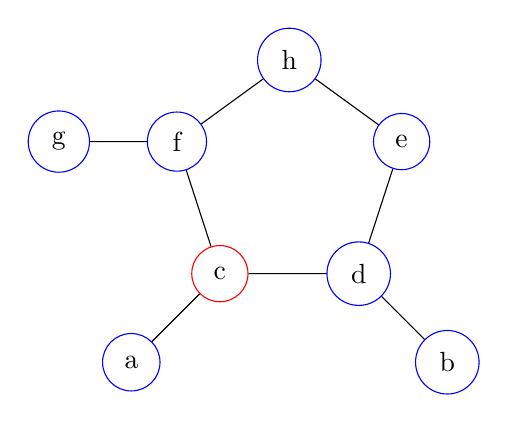
\begin{tikzpicture}[scale=1.5, every node/.style={draw=blue,circle, align=center, inner sep = .5em}]
		\node at (90:1) (h) {h};
		\node at (90-72:1) (e) {e};
		\node at (90-72*2:1) (d) {d};
		\node[draw=red] at (90-72*3:1) (c) {c};
		\node at (90-72*4:1) (f) {f};
		\node at ($(f) + (-1,0)$) (g) {g};
		\node at ($ (c) - (.75,.75) $) (a) {a};
		\node at ($ (d) + (.75,-.75) $) (b) {b};
		\draw (g) -- (f) -- (h) -- (e) -- (d) -- (c) -- (f) (a) -- (c) (b) -- (d);
		\end{tikzpicture}
		\caption{\color{blue}$V\setminus U$ | \color{red} $U$}
	\end{subfigure}
	\begin{subfigure}{.66\textwidth}
		\centering
		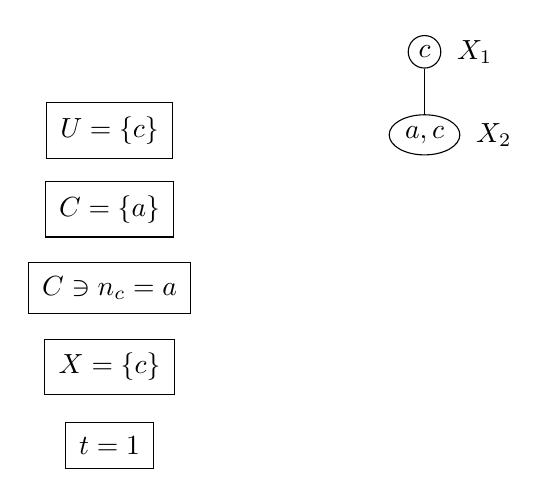
\begin{tikzpicture}[sibling distance = 10em, level distance = 1.5em, scale=2, every node/.style={draw, ellipse, align=center, inner sep = 2}]
		\node[rectangle, inner sep = .5em] at (-2,2.5)   {$U = \{c\}$};
		\node[rectangle, inner sep = .5em] at (-2,2)   {$C = \{a\}$};
		\node[rectangle, inner sep = .5em] at (-2,1) {$X = \{c\}$};
		\node[rectangle, inner sep = .5em] at (-2,.5) {$t = 1$};
		\node[rectangle, inner sep = .5em] at (-2,1.50)  {$C \ni n_c  = a$};
		
		\node[label =0:$X_1$] at (0,3){$c$}
		child{
			node[label=0:$X_2$] {$a,c$}	
		};
		\end{tikzpicture}
		\caption{Tree decomposition $T$}
	\end{subfigure}
\end{figure}

\begin{figure}[H]
	\centering
	\begin{subfigure}{.33\textwidth}
		\centering
		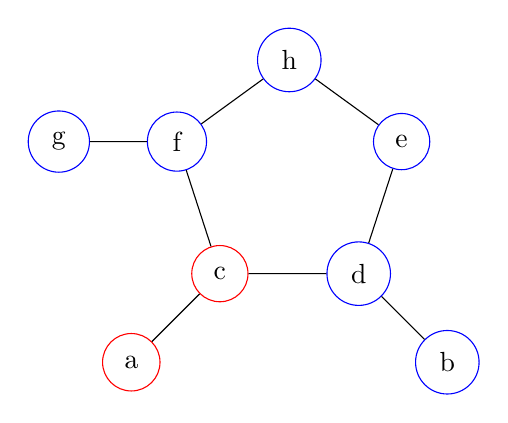
\begin{tikzpicture}[scale=1.5, every node/.style={draw=blue,circle, align=center, inner sep = .5em}]
		\node at (90:1) (h) {h};
		\node at (90-72:1) (e) {e};
		\node at (90-72*2:1) (d) {d};
		\node[draw=red] at (90-72*3:1) (c) {c};
		\node at (90-72*4:1) (f) {f};
		\node at ($(f) + (-1,0)$) (g) {g};
		\node[draw=red] at ($ (c) - (.75,.75) $) (a) {a};
		\node at ($ (d) + (.75,-.75) $) (b) {b};
		\draw (g) -- (f) -- (h) -- (e) -- (d) -- (c) -- (f) (a) -- (c) (b) -- (d);
		\end{tikzpicture}
		\caption{\color{blue}$V\setminus U$ | \color{red} $U$}
	\end{subfigure}
	\begin{subfigure}{.66\textwidth}
		\centering
		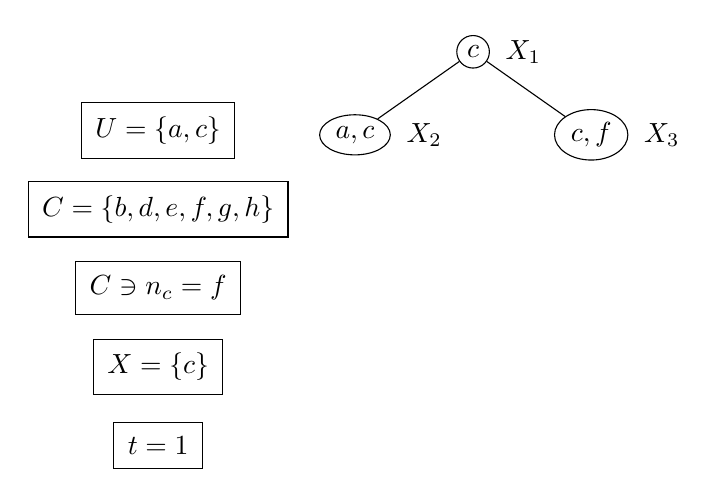
\begin{tikzpicture}[level distance = 1.5em, scale=2, every node/.style={draw, ellipse, align=center, inner sep = 2}]
		\node[rectangle, inner sep = .5em] at (-2,2.5)   {$U = \{a, c\}$};
		\node[rectangle, inner sep = .5em] at (-2,2)   {$C = \{b,d,e,f,g,h\}$};
		\node[rectangle, inner sep = .5em] at (-2,1) {$X = \{c\}$};
		\node[rectangle, inner sep = .5em] at (-2,.5) {$t = 1$};
		\node[rectangle, inner sep = .5em] at (-2,1.50)  {$ C \ni n_c = f$};
		
		\node[label =0:$X_1$] at (0,3){$c$}
		child{
			node[label=0:$X_2$] {$a,c$}	
		}
		child{
			node[label=0:$X_3$] {$c,f$}
		};
		\end{tikzpicture}
		\caption{Tree decomposition $T$}
	\end{subfigure}
\end{figure}

\begin{figure}[H]
	\centering
	\begin{subfigure}{.33\textwidth}
		\centering
		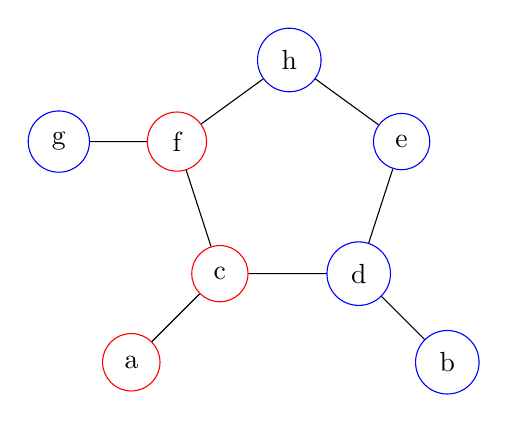
\begin{tikzpicture}[scale=1.5, every node/.style={draw=blue,circle, align=center, inner sep = .5em}]
		\node at (90:1) (h) {h};
		\node at (90-72:1) (e) {e};
		\node at (90-72*2:1) (d) {d};
		\node[draw=red] at (90-72*3:1) (c) {c};
		\node[draw=red] at (90-72*4:1) (f) {f};
		\node at ($(f) + (-1,0)$) (g) {g};
		\node[draw=red] at ($ (c) - (.75,.75) $) (a) {a};
		\node at ($ (d) + (.75,-.75) $) (b) {b};
		\draw (g) -- (f) -- (h) -- (e) -- (d) -- (c) -- (f) (a) -- (c) (b) -- (d);
		\end{tikzpicture}
		\caption{\color{blue}$V\setminus U$ | \color{red} $U$}
	\end{subfigure}
	\begin{subfigure}{.66\textwidth}
		\centering
		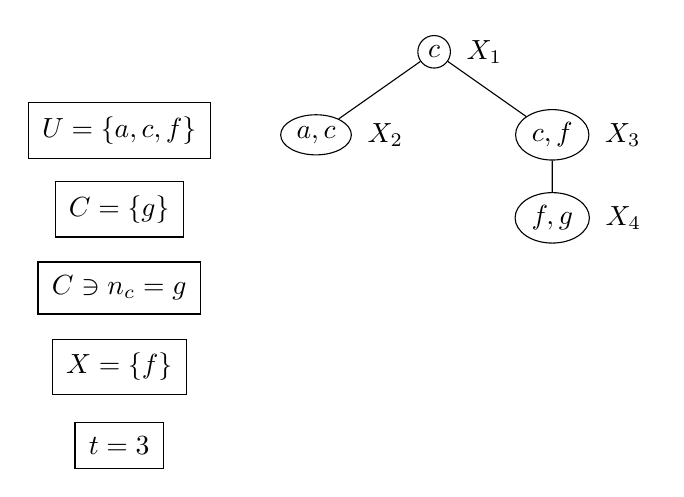
\begin{tikzpicture}[level distance = 1.5em, scale=2, every node/.style={draw, ellipse, align=center, inner sep = 2}]
		\node[rectangle, inner sep = .5em] at (-2,2.5)   {$U = \{a,c,f\}$};
		\node[rectangle, inner sep = .5em] at (-2,2)   {$C = \{g\}$};
		\node[rectangle, inner sep = .5em] at (-2,1) {$X = \{f\}$};
		\node[rectangle, inner sep = .5em] at (-2,.5) {$t = 3$};
		\node[rectangle, inner sep = .5em] at (-2,1.50)  {$ C \ni n_c = g$};
		
		
		\node[label =0:$X_1$] at (0,3){$c$}
		child{
			node[label=0:$X_2$] {$a,c$}	
		}
		child{
			node[label=0:$X_3$] {$c,f$}
			child{
				node[label=0:$X_4$] {$f,g$}	
			}
		};
		
		\end{tikzpicture}
		\caption{Tree decomposition $T$}
	\end{subfigure}
\end{figure}

\begin{figure}[H]
	\centering
	\begin{subfigure}{.33\textwidth}
		\centering
		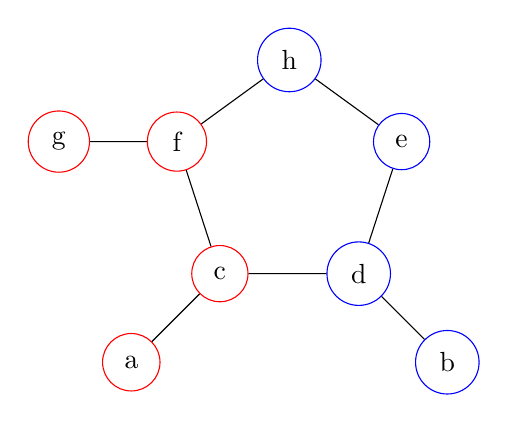
\begin{tikzpicture}[scale=1.5, every node/.style={draw=blue,circle, align=center, inner sep = .5em}]
		\node at (90:1) (h) {h};
		\node at (90-72:1) (e) {e};
		\node at (90-72*2:1) (d) {d};
		\node[draw=red] at (90-72*3:1) (c) {c};
		\node[draw=red] at (90-72*4:1) (f) {f};
		\node[draw=red] at ($(f) + (-1,0)$) (g) {g};
		\node[draw=red] at ($ (c) - (.75,.75) $) (a) {a};
		\node at ($ (d) + (.75,-.75) $) (b) {b};
		\draw (g) -- (f) -- (h) -- (e) -- (d) -- (c) -- (f) (a) -- (c) (b) -- (d);
		\end{tikzpicture}
		\caption{\color{blue}$V\setminus U$ | \color{red} $U$}
	\end{subfigure}
	\begin{subfigure}{.66\textwidth}
		\centering
		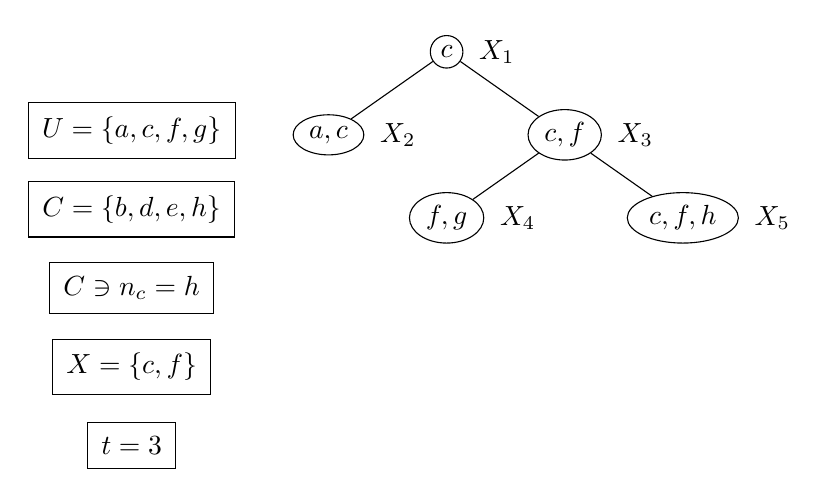
\begin{tikzpicture}[level distance = 1.5em, scale=2, every node/.style={draw, ellipse, align=center, inner sep = 2}]
		\node[rectangle, inner sep = .5em] at (-2,2.5)   {$U = \{a,c,f,g\}$};
		\node[rectangle, inner sep = .5em] at (-2,2)   {$C = \{b,d,e,h\}$};
		\node[rectangle, inner sep = .5em] at (-2,1) {$X = \{c, f\}$};
		\node[rectangle, inner sep = .5em] at (-2,.5) {$t = 3$};
		\node[rectangle, inner sep = .5em] at (-2,1.50)  {$ C \ni n_c = h$};
		
		
		\node[label =0:$X_1$] at (0,3){$c$}
		child{
			node[label=0:$X_2$] {$a,c$}	
		}
		child{
			node[label=0:$X_3$] {$c,f$}
			child{
				node[label=0:$X_4$] {$f,g$}	
			}
			child{
				node[label=0:$X_5$] {$c,f,h$}	
			}
		};
		
		\end{tikzpicture}
		\caption{Tree decomposition $T$}
	\end{subfigure}
\end{figure}

\begin{figure}[H]
	\centering
	\begin{subfigure}{.33\textwidth}
		\centering
		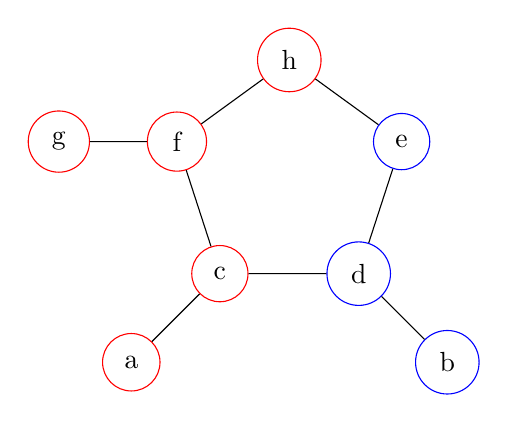
\begin{tikzpicture}[scale=1.5, every node/.style={draw=blue,circle, align=center, inner sep = .5em}]
		\node[draw=red] at (90:1) (h) {h};
		\node at (90-72:1) (e) {e};
		\node at (90-72*2:1) (d) {d};
		\node[draw=red] at (90-72*3:1) (c) {c};
		\node[draw=red] at (90-72*4:1) (f) {f};
		\node[draw=red] at ($(f) + (-1,0)$) (g) {g};
		\node[draw=red] at ($ (c) - (.75,.75) $) (a) {a};
		\node at ($ (d) + (.75,-.75) $) (b) {b};
		\draw (g) -- (f) -- (h) -- (e) -- (d) -- (c) -- (f) (a) -- (c) (b) -- (d);
		\end{tikzpicture}
		\caption{\color{blue}$V\setminus U$ | \color{red} $U$}
	\end{subfigure}
	\begin{subfigure}{.66\textwidth}
		\centering
		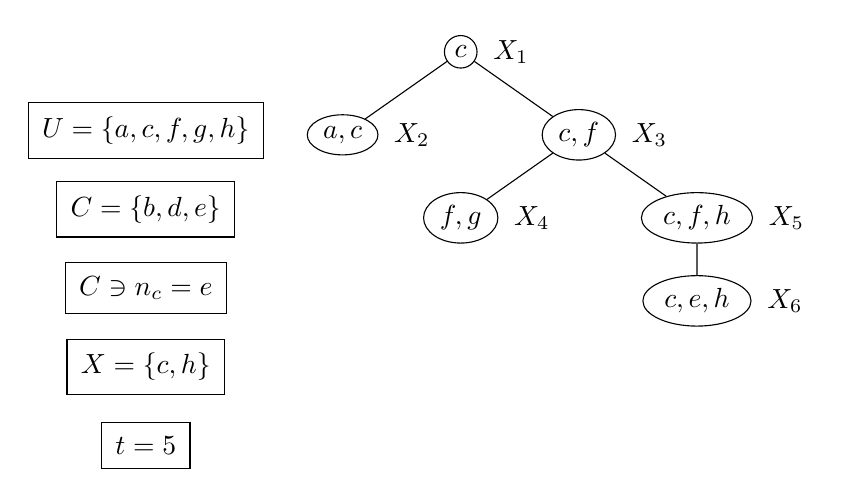
\begin{tikzpicture}[level distance = 1.5em, scale=2, every node/.style={draw, ellipse, align=center, inner sep = 2}]
		\node[rectangle, inner sep = .5em] at (-2,2.5)   {$U = \{a,c,f,g,h\}$};
		\node[rectangle, inner sep = .5em] at (-2,2)   {$C = \{b,d,e\}$};
		\node[rectangle, inner sep = .5em] at (-2,1) {$X = \{c, h\}$};
		\node[rectangle, inner sep = .5em] at (-2,.5) {$t = 5$};
		\node[rectangle, inner sep = .5em] at (-2,1.50)  {$ C \ni n_c = e$};
		
		
		\node[label =0:$X_1$] at (0,3){$c$}
		child{
			node[label=0:$X_2$] {$a,c$}	
		}
		child{
			node[label=0:$X_3$] {$c,f$}
			child{
				node[label=0:$X_4$] {$f,g$}	
			}
			child{
				node[label=0:$X_5$] {$c,f,h$}	
				child {
					node[label=0:$X_6$] {$c,e,h$}	
				}
			}
		};
		
		\end{tikzpicture}
		\caption{Tree decomposition $T$}
	\end{subfigure}
\end{figure}

\begin{figure}[H]
	\centering
	\begin{subfigure}{.33\textwidth}
		\centering
		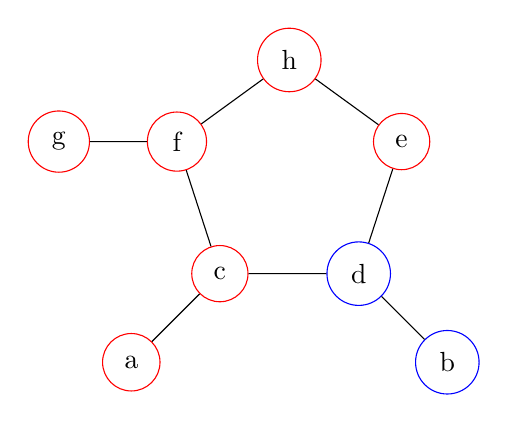
\begin{tikzpicture}[scale=1.5, every node/.style={draw=blue,circle, align=center, inner sep = .5em}]
		\node[draw=red] at (90:1) (h) {h};
		\node[draw=red] at (90-72:1) (e) {e};
		\node at (90-72*2:1) (d) {d};
		\node[draw=red] at (90-72*3:1) (c) {c};
		\node[draw=red] at (90-72*4:1) (f) {f};
		\node[draw=red] at ($(f) + (-1,0)$) (g) {g};
		\node[draw=red] at ($ (c) - (.75,.75) $) (a) {a};
		\node at ($ (d) + (.75,-.75) $) (b) {b};
		\draw (g) -- (f) -- (h) -- (e) -- (d) -- (c) -- (f) (a) -- (c) (b) -- (d);
		\end{tikzpicture}
		\caption{\color{blue}$V\setminus U$ | \color{red} $U$}
	\end{subfigure}
	\begin{subfigure}{.66\textwidth}
		\centering
		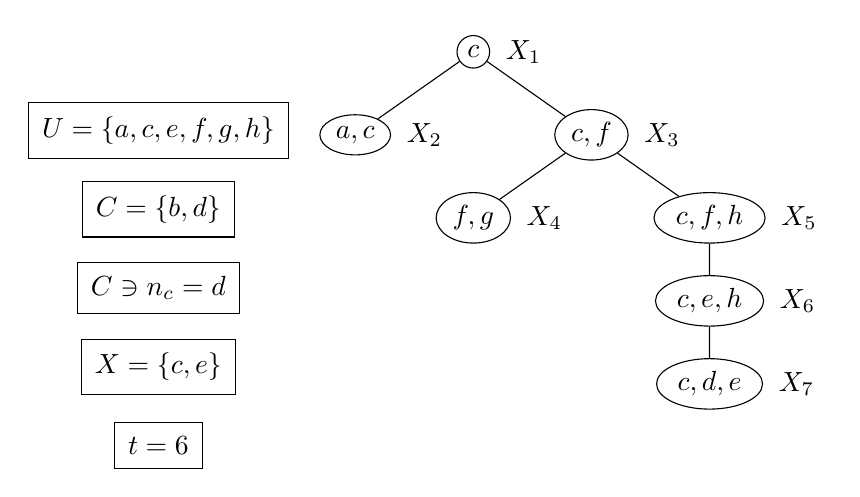
\begin{tikzpicture}[level distance = 1.5em, scale=2, every node/.style={draw, ellipse, align=center, inner sep = 2}]
		\node[rectangle, inner sep = .5em] at (-2,2.5)   {$U = \{a,c,e,f,g,h\}$};
		\node[rectangle, inner sep = .5em] at (-2,2)   {$C = \{b,d\}$};
		\node[rectangle, inner sep = .5em] at (-2,1) {$X = \{c, e\}$};
		\node[rectangle, inner sep = .5em] at (-2,.5) {$t = 6$};
		\node[rectangle, inner sep = .5em] at (-2,1.50)  {$ C \ni n_c = d$};
		
		
		\node[label =0:$X_1$] at (0,3){$c$}
		child{
			node[label=0:$X_2$] {$a,c$}	
		}
		child{
			node[label=0:$X_3$] {$c,f$}
			child{
				node[label=0:$X_4$] {$f,g$}	
			}
			child{
				node[label=0:$X_5$] {$c,f,h$}	
				child {
					node[label=0:$X_6$] {$c,e,h$}
					child{
						node[label=0:$X_7$] {$c,d,e$}	
					}	
				}
			}
		};
		
		\end{tikzpicture}
		\caption{Tree decomposition $T$}
	\end{subfigure}
\end{figure}

\begin{figure}[H]
	\centering
	\begin{subfigure}{.33\textwidth}
		\centering
		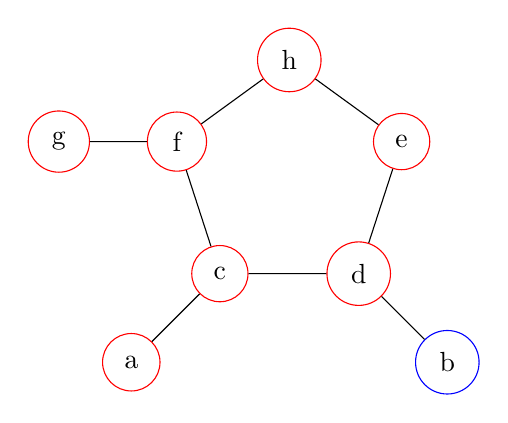
\begin{tikzpicture}[scale=1.5, every node/.style={draw=blue,circle, align=center, inner sep = .5em}]
		\node[draw=red] at (90:1) (h) {h};
		\node[draw=red] at (90-72:1) (e) {e};
		\node[draw=red] at (90-72*2:1) (d) {d};
		\node[draw=red] at (90-72*3:1) (c) {c};
		\node[draw=red] at (90-72*4:1) (f) {f};
		\node[draw=red] at ($(f) + (-1,0)$) (g) {g};
		\node[draw=red] at ($ (c) - (.75,.75) $) (a) {a};
		\node at ($ (d) + (.75,-.75) $) (b) {b};
		\draw (g) -- (f) -- (h) -- (e) -- (d) -- (c) -- (f) (a) -- (c) (b) -- (d);
		\end{tikzpicture}
		\caption{\color{blue}$V\setminus U$ | \color{red} $U$}
	\end{subfigure}
	\begin{subfigure}{.66\textwidth}
		\centering
		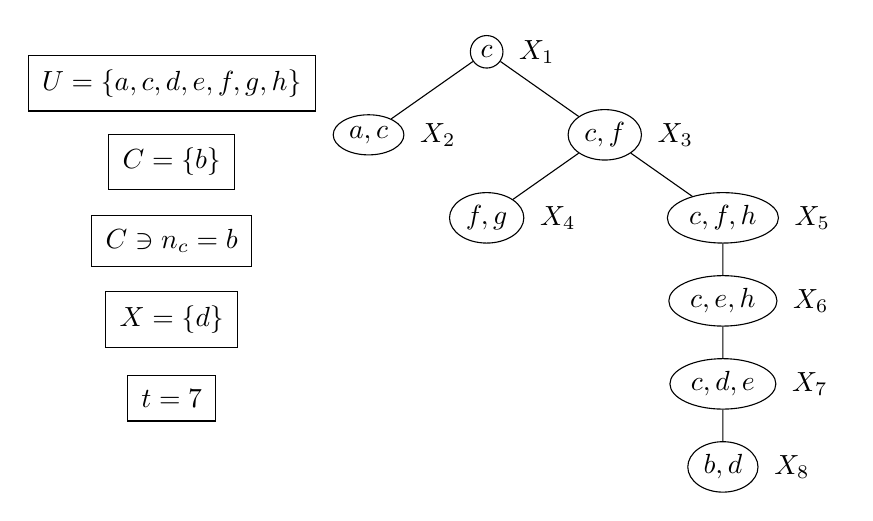
\begin{tikzpicture}[level distance = 1.5em, scale=2, every node/.style={draw, ellipse, align=center, inner sep = 2}]
		\node[rectangle, inner sep = .5em] at (-2,2.5)   {$U = \{a,c,d,e,f,g,h\}$};
		\node[rectangle, inner sep = .5em] at (-2,2)   {$C = \{b\}$};
		\node[rectangle, inner sep = .5em] at (-2,1) {$X = \{d\}$};
		\node[rectangle, inner sep = .5em] at (-2,.5) {$t = 7$};
		\node[rectangle, inner sep = .5em] at (-2,1.50)  {$ C \ni n_c = b$};
		
		
		\node[label =0:$X_1$] at (0,2.7){$c$}
		child{
			node[label=0:$X_2$] {$a,c$}	
		}
		child{
			node[label=0:$X_3$] {$c,f$}
			child{
				node[label=0:$X_4$] {$f,g$}	
			}
			child{
				node[label=0:$X_5$] {$c,f,h$}	
				child {
					node[label=0:$X_6$] {$c,e,h$}
					child{
						node[label=0:$X_7$] {$c,d,e$}
						child{
							node[label=0:$X_8$] {$b,d$}	
						}
					}	
				}
			}
		};
		
		\end{tikzpicture}
		\caption{Tree decomposition $T$}
	\end{subfigure}
\end{figure}
\small
\begin{align*}
\begin{array}{l|ccccccccc}
\text{step}	&0			&1		&2				&3			&4				&5				&6					&7					&\text{Result}\\\hline
U			&\emptyset	&\{c\}	&\{a,c\}		&\{a,c,f\}	&\{a,c,f,g\}	&\{a,c,f,g,h\}	&\{a,c,e,f,g,h\}	&\tiny\{a,c,d,e,f,g,h\}	&	V\\
C			&V			&\{a\}	&\{b,d,e,f,g,h\}&\{g\}		&\{b,d,e,h\}	&\{b,d,e\}		&\{b,d\}			&\{b\}				&\emptyset\\
C\ni n_C	&c			&a		&f				&g			&h				&e				&d					&b					&/\\
X			&\emptyset	&\{c\}	&\{c\}			&\{f\}		&\{c,f\}		&\{c,h\}		&\{c,e\}			&\{d\}				&\emptyset\\
t			&/			&1		&1				&3			&3				&5				&6					&7					&/
\end{array}
\end{align*}
\normalsize
\begin{figure}[H]
	\centering
	\begin{subfigure}{.45\textwidth}
		\centering
		\begin{tikzpicture}[scale=2, every node/.style={draw,circle, align=center, inner sep = .5em}]
		\node at (90:1) (h) {h};
		\node at (90-72:1) (e) {e};
		\node at (90-72*2:1) (d) {d};
		\node at (90-72*3:1) (c) {c};
		\node at (90-72*4:1) (f) {f};
		\node at ($(f) + (-1,0)$) (g) {g};
		\node at ($ (c) - (.75,.75) $) (a) {a};
		\node at ($ (d) + (.75,-.75) $) (b) {b};
		\draw (g) -- (f) -- (h) -- (e) -- (d) -- (c) -- (f) (a) -- (c) (b) -- (d);
		\end{tikzpicture}
		\caption{Graph $G$}
	\end{subfigure}
	\begin{subfigure}{.45\textwidth}
		\centering
		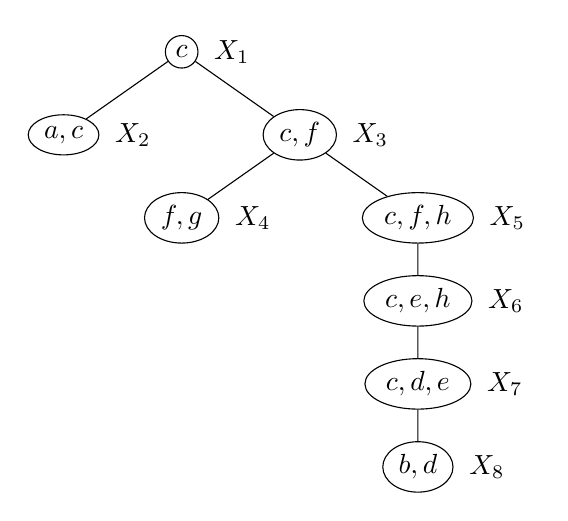
\begin{tikzpicture}[level distance = 1.5em, scale=2, every node/.style={draw, ellipse, align=center, inner sep = 2}]
		\node[label =0:$X_1$] {$c$}
		child{
			node[label=0:$X_2$] {$a,c$}	
		}
		child{
			node[label=0:$X_3$] {$c,f$}
			child{
				node[label=0:$X_4$] {$f,g$}	
			}
			child{
				node[label=0:$X_5$] {$c,f,h$}	
				child {
					node[label=0:$X_6$] {$c,e,h$}
					child{
						node[label=0:$X_7$] {$c,d,e$}
						child{
							node[label=0:$X_8$] {$b,d$}	
						}
					}	
				}
			}
		};
		
		\end{tikzpicture}
		\caption{Tree decomposition $T$}
	\end{subfigure}
	\caption{Result}
\end{figure}
\pagebreak
\subsection{b}
\begin{figure}[H]
	\centering
	\begin{subfigure}{.45\textwidth}
		\centering
		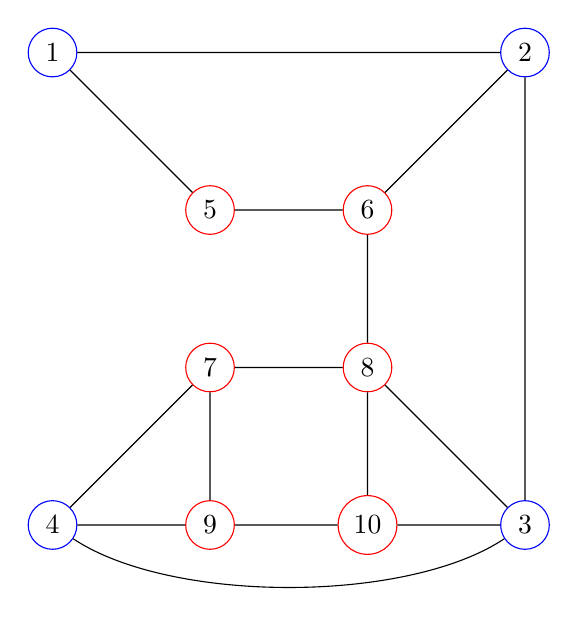
\begin{tikzpicture}[scale=2, every node/.style={draw=blue, circle, align=center}]
		\node at (0,3) (1) {1};
		\node at (3,3) (2) {2};
		\node at (3,0) (3) {3};
		\node at (0,0) (4) {4};
		\node[draw=red] at (1,2) (5) {5};
		\node[draw=red] at (2,2) (6) {6};
		\node[draw=red] at (1,1) (7) {7};
		\node[draw=red] at (2,1) (8) {8};
		\node[draw=red] at (1,0) (9) {9};
		\node[draw=red] at (2,0) (10) {10};
		\draw (1) -- (2) -- (3) -- (10) -- (9) -- (7) -- (8) -- (6) -- (5) -- (1) (6)--(2) (10)--(8) -- (3) (9) -- (4) -- (7);
		\draw (3) .. controls ($(3)!.25!(4)+(0,-.5)$) and ($(3)!.75!(4)+(0,-.5)$)  .. (4);
		\end{tikzpicture}
		\caption{$U=X=\{5,6,7,8,9,10\}$}
	\end{subfigure}
	\begin{subfigure}{.45\textwidth}
		\centering
		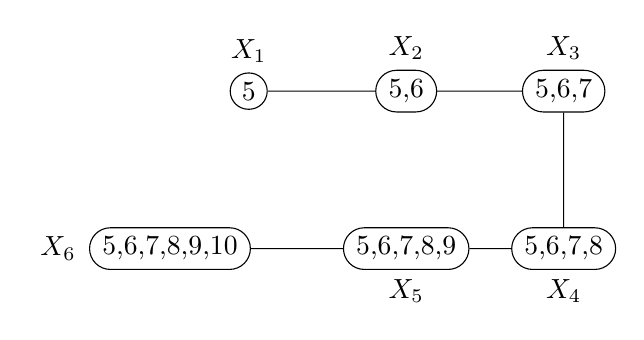
\begin{tikzpicture}[scale=2, every node/.style={draw, rounded rectangle, align=center}]
		\node[label=90:$X_1$]  at (0,1) (1) {5};
		\node[label=90:$X_2$]  at (1,1) (2) {5,6};
		\node[label=90:$X_3$]  at (2,1) (3) {5,6,7};
		\node[label=-90:$X_4$] at (2,0) (4) {5,6,7,8};
		\node[label=-90:$X_5$] at (1,0) (5) {5,6,7,8,9};
		\node[label=180:$X_6$] at (-.5,0) (6) {5,6,7,8,9,10};
		\draw (1) -- (2) -- (3) -- (4) -- (5) -- (6);
		\end{tikzpicture}
		\caption{$C=\{1,2,3,4\}$}
	\end{subfigure}
\end{figure}
$X = \{ 5,6,7,8,9,10 \}$ ist nicht $w+1=3$ verbunden, da $Y=\{7,9,10\}$ und $Z=\{5,6,8\}$ durch $S=\{8,3\}$ separierbar ist. Weiter gilt:
\begin{align*}
\begin{array}{ccccccc}
|S|& < &|Y|&=&|Z| &\leq &w + 1\\
2& < &3&=&3 &\leq &3
\end{array}
\end{align*} 
$S' = S\cap (Y\cup Z \cup C) = \{ 3,8 \}$ und somit $X_7 = X \cup S' = \{3,5,6,7,8,9,10\}$

\begin{figure}[H]
	\centering
	\begin{subfigure}{.45\textwidth}
		\centering
		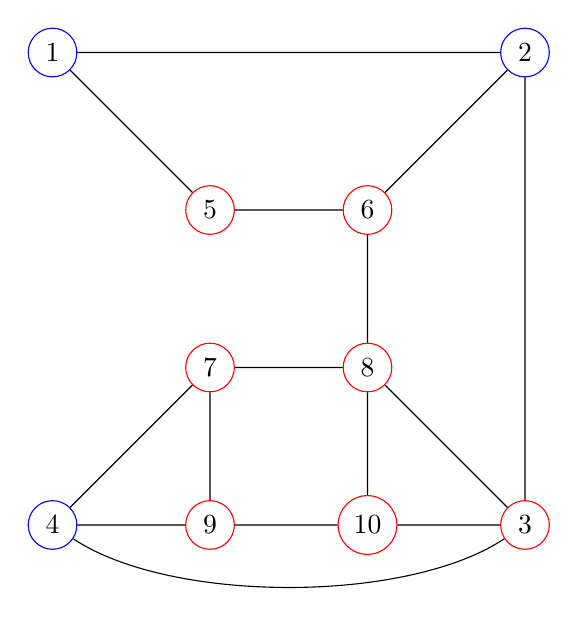
\begin{tikzpicture}[scale=2, every node/.style={draw=blue, circle, align=center}]
		\node at (0,3) (1) {1};
		\node at (3,3) (2) {2};
		\node[draw=red] at (3,0) (3) {3};
		\node at (0,0) (4) {4};
		\node[draw=red] at (1,2) (5) {5};
		\node[draw=red] at (2,2) (6) {6};
		\node[draw=red] at (1,1) (7) {7};
		\node[draw=red] at (2,1) (8) {8};
		\node[draw=red] at (1,0) (9) {9};
		\node[draw=red] at (2,0) (10) {10};
		\draw (1) -- (2) -- (3) -- (10) -- (9) -- (7) -- (8) -- (6) -- (5) -- (1) (6)--(2) (10)--(8) -- (3) (9) -- (4) -- (7);
		\draw (3) .. controls ($(3)!.25!(4)+(0,-.5)$) and ($(3)!.75!(4)+(0,-.5)$)  .. (4);
		\end{tikzpicture}

	\end{subfigure}
	\begin{subfigure}{.45\textwidth}
		\centering
		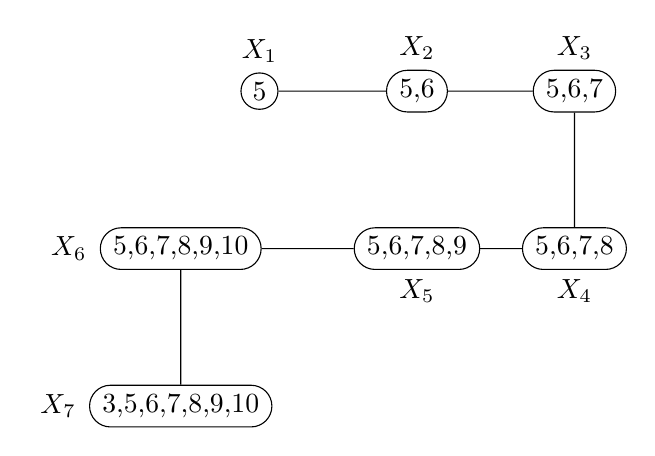
\begin{tikzpicture}[scale=2, every node/.style={draw, rounded rectangle, align=center}]
		\node[label=90:$X_1$]  at (0,1) (1) {5};
		\node[label=90:$X_2$]  at (1,1) (2) {5,6};
		\node[label=90:$X_3$]  at (2,1) (3) {5,6,7};
		\node[label=-90:$X_4$] at (2,0) (4) {5,6,7,8};
		\node[label=-90:$X_5$] at (1,0) (5) {5,6,7,8,9};
		\node[label=180:$X_6$] at (-.5,0) (6) {5,6,7,8,9,10};
		\node[label=180:$X_7$] at (-.5,-1) (7) {3,5,6,7,8,9,10};
		\draw (1) -- (2) -- (3) -- (4) -- (5) -- (6) -- (7);
		\end{tikzpicture}

	\end{subfigure}
\end{figure}

\begin{figure}[H]
	\centering
	\begin{subfigure}{.45\textwidth}
		\centering
		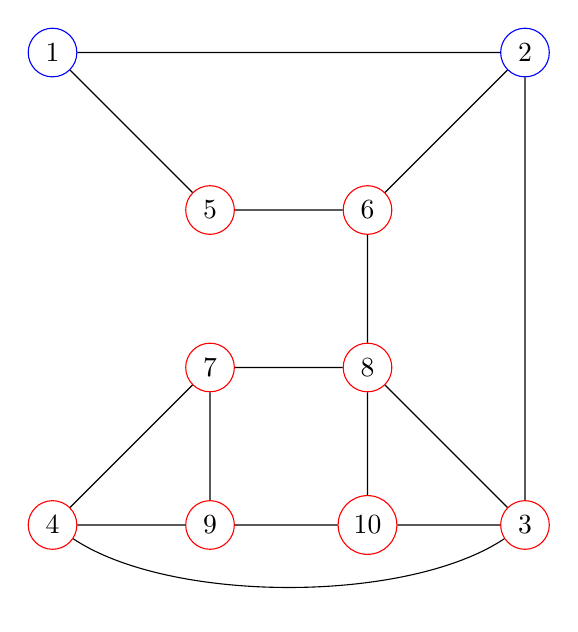
\begin{tikzpicture}[scale=2, every node/.style={draw=blue, circle, align=center}]
		\node at (0,3) (1) {1};
		\node at (3,3) (2) {2};
		\node[draw=red] at (3,0) (3) {3};
		\node[draw=red] at (0,0) (4) {4};
		\node[draw=red] at (1,2) (5) {5};
		\node[draw=red] at (2,2) (6) {6};
		\node[draw=red] at (1,1) (7) {7};
		\node[draw=red] at (2,1) (8) {8};
		\node[draw=red] at (1,0) (9) {9};
		\node[draw=red] at (2,0) (10) {10};
		\draw (1) -- (2) -- (3) -- (10) -- (9) -- (7) -- (8) -- (6) -- (5) -- (1) (6)--(2) (10)--(8) -- (3) (9) -- (4) -- (7);
		\draw (3) .. controls ($(3)!.25!(4)+(0,-.5)$) and ($(3)!.75!(4)+(0,-.5)$)  .. (4);
		\end{tikzpicture}
		\caption{$U=\{3,5,6,7,8,9,10\},~X=\{3,7,9\}$}
	\end{subfigure}
	\begin{subfigure}{.45\textwidth}
		\centering
		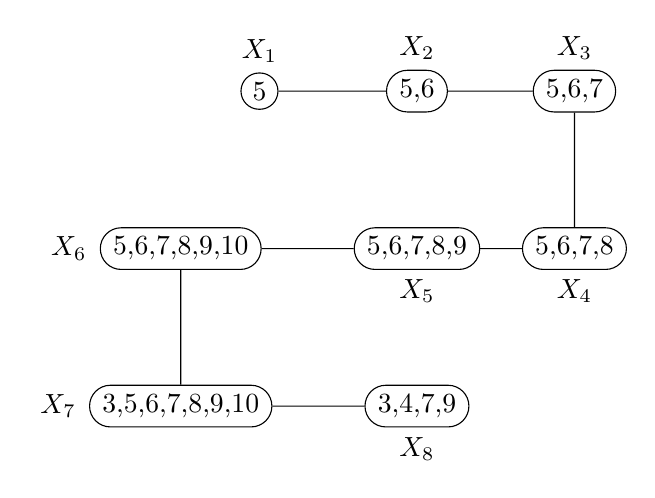
\begin{tikzpicture}[scale=2, every node/.style={draw, rounded rectangle, align=center}]
		\node[label=90:$X_1$]  at (0,1) (1) {5};
		\node[label=90:$X_2$]  at (1,1) (2) {5,6};
		\node[label=90:$X_3$]  at (2,1) (3) {5,6,7};
		\node[label=-90:$X_4$] at (2,0) (4) {5,6,7,8};
		\node[label=-90:$X_5$] at (1,0) (5) {5,6,7,8,9};
		\node[label=180:$X_6$] at (-.5,0) (6) {5,6,7,8,9,10};
		\node[label=180:$X_7$] at (-.5,-1) (7) {3,5,6,7,8,9,10};
		\node[label=-90:$X_8$] at (1,-1) (8) {3,4,7,9};
		\draw (1) -- (2) -- (3) -- (4) -- (5) -- (6) -- (7) -- (8);
		\end{tikzpicture}
		\caption{$C=\{4\}$}
	\end{subfigure}
\end{figure}

\begin{figure}[H]
	\centering
	\begin{subfigure}{.45\textwidth}
		\centering
		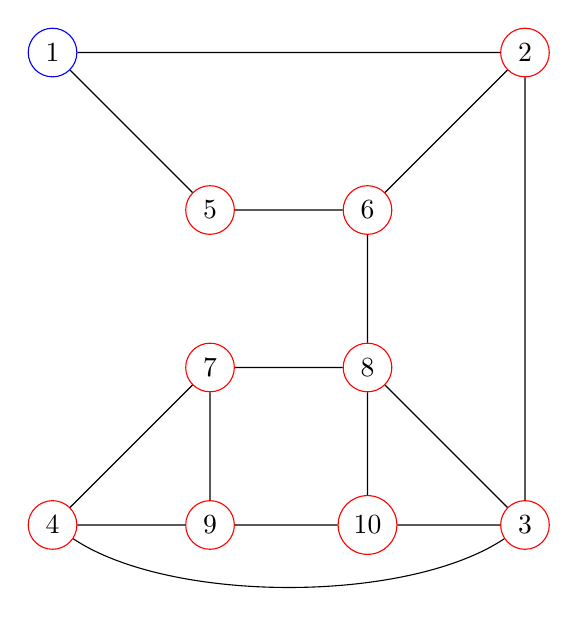
\begin{tikzpicture}[scale=2, every node/.style={draw=blue, circle, align=center}]
		\node at (0,3) (1) {1};
		\node[draw=red] at (3,3) (2) {2};
		\node[draw=red] at (3,0) (3) {3};
		\node[draw=red] at (0,0) (4) {4};
		\node[draw=red] at (1,2) (5) {5};
		\node[draw=red] at (2,2) (6) {6};
		\node[draw=red] at (1,1) (7) {7};
		\node[draw=red] at (2,1) (8) {8};
		\node[draw=red] at (1,0) (9) {9};
		\node[draw=red] at (2,0) (10) {10};
		\draw (1) -- (2) -- (3) -- (10) -- (9) -- (7) -- (8) -- (6) -- (5) -- (1) (6)--(2) (10)--(8) -- (3) (9) -- (4) -- (7);
		\draw (3) .. controls ($(3)!.25!(4)+(0,-.5)$) and ($(3)!.75!(4)+(0,-.5)$)  .. (4);
		\end{tikzpicture}
		\caption{$U=\{3,4,5,6,7,8,9,10\},~X=\{3,5,6\}$}
	\end{subfigure}
	\begin{subfigure}{.45\textwidth}
		\centering
		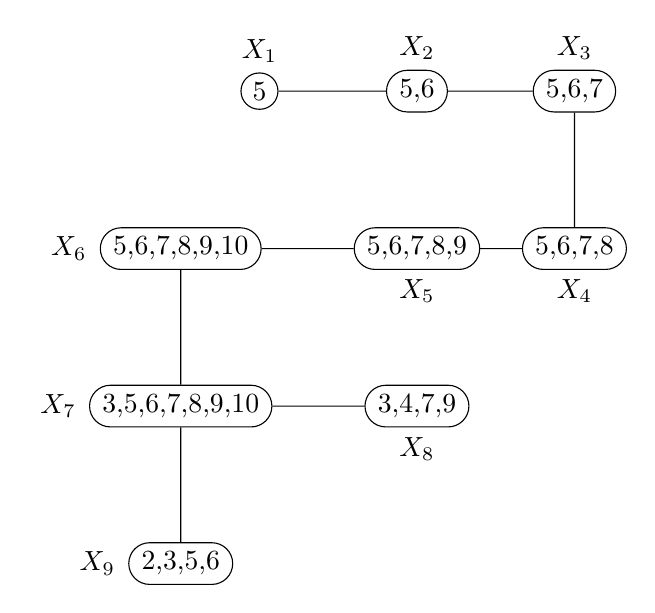
\begin{tikzpicture}[scale=2, every node/.style={draw, rounded rectangle, align=center}]
		\node[label=90:$X_1$]  at (0,1) (1) {5};
		\node[label=90:$X_2$]  at (1,1) (2) {5,6};
		\node[label=90:$X_3$]  at (2,1) (3) {5,6,7};
		\node[label=-90:$X_4$] at (2,0) (4) {5,6,7,8};
		\node[label=-90:$X_5$] at (1,0) (5) {5,6,7,8,9};
		\node[label=180:$X_6$] at (-.5,0) (6) {5,6,7,8,9,10};
		\node[label=180:$X_7$] at (-.5,-1) (7) {3,5,6,7,8,9,10};
		\node[label=-90:$X_8$] at (1,-1) (8) {3,4,7,9};
		\node[label=180:$X_9$] at (-.5,-2) (9) {2,3,5,6};
		\draw (1) -- (2) -- (3) -- (4) -- (5) -- (6) -- (7) -- (8) (7)--(9);
		\end{tikzpicture}
		\caption{$C=\{1,2\}$}
	\end{subfigure}
\end{figure}

\begin{figure}[H]
	\centering
	\begin{subfigure}{.45\textwidth}
		\centering
		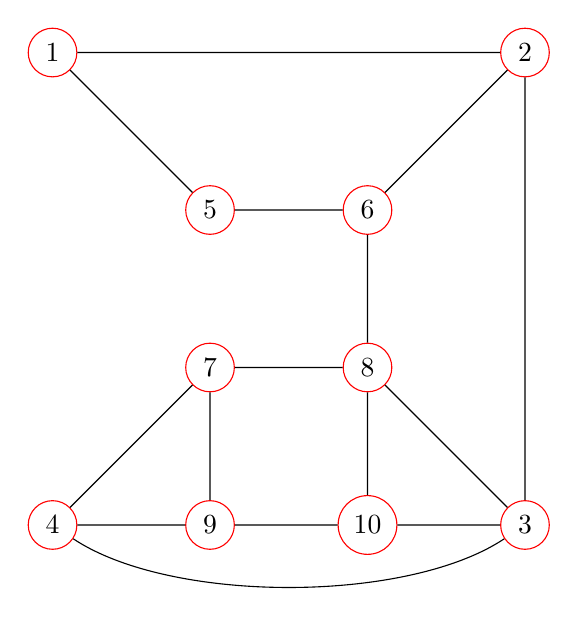
\begin{tikzpicture}[scale=2, every node/.style={draw=blue, circle, align=center}]
		\node[draw=red] at (0,3) (1) {1};
		\node[draw=red] at (3,3) (2) {2};
		\node[draw=red] at (3,0) (3) {3};
		\node[draw=red] at (0,0) (4) {4};
		\node[draw=red] at (1,2) (5) {5};
		\node[draw=red] at (2,2) (6) {6};
		\node[draw=red] at (1,1) (7) {7};
		\node[draw=red] at (2,1) (8) {8};
		\node[draw=red] at (1,0) (9) {9};
		\node[draw=red] at (2,0) (10) {10};
		\draw (1) -- (2) -- (3) -- (10) -- (9) -- (7) -- (8) -- (6) -- (5) -- (1) (6)--(2) (10)--(8) -- (3) (9) -- (4) -- (7);
		\draw (3) .. controls ($(3)!.25!(4)+(0,-.5)$) and ($(3)!.75!(4)+(0,-.5)$)  .. (4);
		\end{tikzpicture}
		\caption{$U=\{2,3,4,5,6,7,8,9,10\},~X=\{2,5\}$}
	\end{subfigure}
	\begin{subfigure}{.45\textwidth}
		\centering
		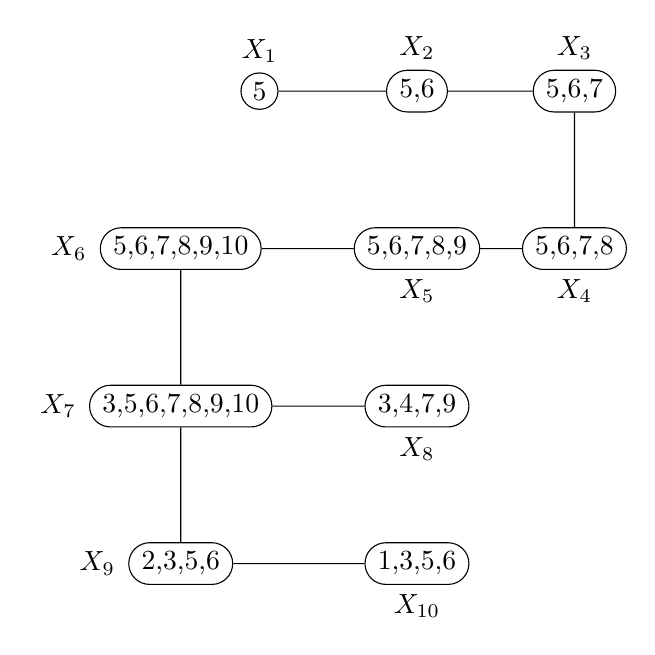
\begin{tikzpicture}[scale=2, every node/.style={draw, rounded rectangle, align=center}]
		\node[label=90:$X_1$]  at (0,1) (1) {5};
		\node[label=90:$X_2$]  at (1,1) (2) {5,6};
		\node[label=90:$X_3$]  at (2,1) (3) {5,6,7};
		\node[label=-90:$X_4$] at (2,0) (4) {5,6,7,8};
		\node[label=-90:$X_5$] at (1,0) (5) {5,6,7,8,9};
		\node[label=180:$X_6$] at (-.5,0) (6) {5,6,7,8,9,10};
		\node[label=180:$X_7$] at (-.5,-1) (7) {3,5,6,7,8,9,10};
		\node[label=-90:$X_8$] at (1,-1) (8) {3,4,7,9};
		\node[label=180:$X_9$] at (-.5,-2) (9) {2,3,5,6};
		\node[label=-90:$X_{10}$] at (1,-2) (10) {1,3,5,6};
		\draw (1) -- (2) -- (3) -- (4) -- (5) -- (6) -- (7) -- (8) (7)--(9)--(10);
		\end{tikzpicture}
		\caption{$C=\{1\}$}
	\end{subfigure}
\end{figure}

\small
\begin{align*}
\begin{array}{l|ccccccc}
\text{step}	&\ldots	&7			&8						&9						&10\\\hline
U			&&\{5,6,7,8,9,10\}	&\{3,5,6,7,8,9,10\}		&\{3,4,5,6,7,8,9,10\}	&\{2,3,4,5,6,7,8,9,10\}	\\
C			&&\{1,2,3,4\}		&\{4\}					&\{1,2\}				&\{1\}		\\
C\ni n_C	&&/					&4						&2						&1		\\
X			&&\{5,6,7,8,9,10\}	&\{3,7,9\}				&\{3,5,6\}				&\{2,5\}		\\
t			&&6					&7						&7						&9			\\
Y			&&\{7,9,10\}		&/						&/						&/\\
Z			&&\{5,6,8\}			&/						&/						&/\\
S			&&\{3,8\}			&/						&/						&/
\end{array}
\end{align*}
\normalsize

\end{document}